\documentclass[
  onecolumn]{article}
\usepackage{amsmath,amssymb}
\usepackage{lmodern}


\usepackage{setspace}
\usepackage{iftex}
\ifPDFTeX
  \usepackage[T1]{fontenc}
  \usepackage[utf8]{inputenc}
  \usepackage{textcomp} % provide euro and other symbols
\else % if luatex or xetex
  \usepackage{unicode-math}
  \defaultfontfeatures{Scale=MatchLowercase}
  \defaultfontfeatures[\rmfamily]{Ligatures=TeX,Scale=1}
\fi
% Use upquote if available, for straight quotes in verbatim environments
\IfFileExists{upquote.sty}{\usepackage{upquote}}{}
\IfFileExists{microtype.sty}{% use microtype if available
  \usepackage[]{microtype}
  \UseMicrotypeSet[protrusion]{basicmath} % disable protrusion for tt fonts
}{}
\makeatletter
\@ifundefined{KOMAClassName}{% if non-KOMA class
  \IfFileExists{parskip.sty}{%
    \usepackage{parskip}
  }{% else
    \setlength{\parindent}{0pt}
    \setlength{\parskip}{6pt plus 2pt minus 1pt}}
}{% if KOMA class
  \KOMAoptions{parskip=half}}
\makeatother
\usepackage{xcolor}
\IfFileExists{xurl.sty}{\usepackage{xurl}}{} % add URL line breaks if available
\IfFileExists{bookmark.sty}{\usepackage{bookmark}}{\usepackage{hyperref}}
\hypersetup{
  pdftitle={Comparing Treatments for Amblyopia with a Synaptic Plasticity Model},
  pdfauthor={Brian S. Blais},
  colorlinks=true,
  linkcolor={blue},
  filecolor={blue},
  citecolor={blue},
  urlcolor={blue},
  pdfcreator={LaTeX via pandoc}}
\urlstyle{same} % disable monospaced font for URLs
\usepackage{graphicx}
\graphicspath{{resources/}}
\makeatletter
\def\maxwidth{\ifdim\Gin@nat@width>\linewidth\linewidth\else\Gin@nat@width\fi}
\def\maxheight{\ifdim\Gin@nat@height>\textheight\textheight\else\Gin@nat@height\fi}
\makeatother
% Scale images if necessary, so that they will not overflow the page
% margins by default, and it is still possible to overwrite the defaults
% using explicit options in \includegraphics[width, height, ...]{}
\setkeys{Gin}{width=\maxwidth,height=\maxheight,keepaspectratio}
% Set default figure placement to htbp
\makeatletter
\def\fps@figure{htbp}
\makeatother
\setlength{\emergencystretch}{3em} % prevent overfull lines
\providecommand{\tightlist}{%
  \setlength{\itemsep}{0pt}\setlength{\parskip}{0pt}}
\setcounter{secnumdepth}{2}
\ifLuaTeX
  \usepackage{selnolig}  % disable illegal ligatures
\fi
\newlength{\cslhangindent}
\setlength{\cslhangindent}{1.5em}
\newlength{\csllabelwidth}
\setlength{\csllabelwidth}{3em}
\newenvironment{CSLReferences}[2] % #1 hanging-ident, #2 entry spacing
 {% don't indent paragraphs
  \setlength{\parindent}{0pt}
  % turn on hanging indent if param 1 is 1
  \ifodd #1 \everypar{\setlength{\hangindent}{\cslhangindent}}\ignorespaces\fi
  % set entry spacing
  \ifnum #2 > 0
  \setlength{\parskip}{#2\baselineskip}
  \fi
 }%
 {}
\usepackage{calc}
\newcommand{\CSLBlock}[1]{#1\hfill\break}
\newcommand{\CSLLeftMargin}[1]{\parbox[t]{\csllabelwidth}{#1}}
\newcommand{\CSLRightInline}[1]{\parbox[t]{\linewidth - \csllabelwidth}{#1}\break}
\newcommand{\CSLIndent}[1]{\hspace{\cslhangindent}#1}

\title{Comparing Treatments for Amblyopia with a Synaptic Plasticity
Model}
\author{Brian S. Blais}
\date{}

\topmargin=-0.5in
\textheight=9.2in
\oddsidemargin=-0.2in
\evensidemargin=0.0in
\textwidth=6.90in
\parindent=30pt
\parskip=3pt
\headheight=15pt
\reversemarginpar
\marginparwidth=.75in
%
%
\renewcommand{\theequation}{\thesection.\arabic{equation}}
\newcommand{\doublesp}{\renewcommand{\baselinestretch}{2.0}}
\newcommand{\mediumsp}{\renewcommand{\baselinestretch}{1.6}}
\newcommand{\singlesp}{\renewcommand{\baselinestretch}{1.0}}
%
\pagestyle{myheadings}
\thispagestyle{empty}
\markright{\today}
\newlength{\figlen}
\setlength{\figlen}{3.7in}

\input stddefs.tex


\begin{document}
\maketitle

{
\hypersetup{linkcolor=}
\setcounter{tocdepth}{3}
\tableofcontents
}
\setstretch{1.5}
\hypertarget{preface}{%
\section*{Preface}\label{preface}}
\addcontentsline{toc}{section}{Preface}

These notes are produced with a combination of Obsidian
(\url{https://obsidian.md}), pandoc (\url{https://pandoc.org}), and some
self-styled python scripts ()

\hypertarget{software-installation}{%
\subsection*{Software Installation}\label{software-installation}}
\addcontentsline{toc}{subsection}{Software Installation}

The software is Python-based with parts written in Cython.

\begin{itemize}
\tightlist
\item
  Download the Anaconda Distribution of Python:
\end{itemize}

\url{https://www.anaconda.com/products/individual\#downloads}

\begin{itemize}
\tightlist
\item
  Download and extract the \emph{PlasticNet} package at:
\end{itemize}

\url{https://github.com/bblais/Plasticnet/archive/refs/heads/master.zip}

\begin{itemize}
\tightlist
\item
  Run the script \texttt{install.py}
\end{itemize}

\hypertarget{printable-versions}{%
\subsection*{Printable Versions}\label{printable-versions}}
\addcontentsline{toc}{subsection}{Printable Versions}

Printable versions of this report can be found on the GitHub site for
this project,

\begin{itemize}
\tightlist
\item
  \href{}{Microsoft Word version}
\item
  \href{}{PDF version}
\end{itemize}

\hypertarget{introduction}{%
\section{Introduction}\label{introduction}}

These notes are an exploration of the problem of modeling Amblyopia and
its various treatments from an approach using synaptic plasticity
models. The process will involve constructing a simplified mechanism for
the development of amblyopic deficits and subsequently modeling both
monocular and binocular treatment protocols. The goal is to understand
the dynamics of the recovery from amblyopic deficits for the different
treatment protocols, to compare the effectiveness of each protocol, and
to explore their limitations. Ideally we would like to use these models
to inform future protocol parameters and perhaps suggest novel
treatments for amblyopia.

In this part we will explore the clinical basis for amblyopia and its
treatments. In the (\textbf{sec-models-of-development?}) and
(\textbf{sec-models-of-treatments?}) we will explore the models that are
used to describe the deficits from amblyopia and their treatment,
respectively.

\hypertarget{what-is-amblyopia}{%
\subsection{What is Amblyopia?}\label{what-is-amblyopia}}

Amblyopia is the most common cause of vision loss in children, caused by
refractive errors or misalignment of the eyes (Zárate and Tejedor,
2007).

\begin{itemize}
\tightlist
\item
  Visual acuity
\item
  Contrast sensitivity
\item
  Color
\item
  Depth (Stereopsis)
\item
  Motion
\item
  Visual fields
\end{itemize}

\hypertarget{how-is-it-treated}{%
\subsection{How is it Treated?}\label{how-is-it-treated}}

The current primary treatment is described in the \emph{Amblyopia
Preferred Practice Method} (Wallace et al., 2018). Treatments are
divided into two broad categories, monocular and binocular treatments.
Monocular treatments produce a competition between the two eyes by
treating only the fellow eye to that the amblyopic eye recovers.
Binocular treatments seek to stimulate both eyes in such a way that
binocular mechanisms can produce a recovery in the amblyopic eye.

\hypertarget{monocular-treatments}{%
\subsubsection{Monocular Treatments}\label{monocular-treatments}}

The most common treatment includes

\begin{enumerate}
\def\labelenumi{\arabic{enumi}.}
\tightlist
\item
  the optical correction of significant refractive errors
\item
  patching the dominant eye which forces the visual input to come from
  only the amblyopic eye.
\end{enumerate}

Although patching is the most common method of treatment, other methods
are described including pharmacology and technology (Gao et al., 2018;
Glaser et al., 2002; Jonathan M. Holmes et al., 2016b; Jonathan M.
Holmes et al., 2016a; Kelly et al., 2016; Li et al., 2015; Zárate and
Tejedor, 2007). These include,

\begin{enumerate}
\def\labelenumi{\arabic{enumi}.}
\setcounter{enumi}{2}
\tightlist
\item
  Pharmacological treatment with atropine drops in the fellow eye
\end{enumerate}

Each of these treatments only directly applies to the fellow eye and the
amblyopic eye is left untouched.

\hypertarget{binocular-treatments}{%
\subsubsection{Binocular Treatments}\label{binocular-treatments}}

There are some treatments which are administered to both eyes, making
them binocular treatments. The one that we will be addressing here use
virtual reality headsets(Xiao et al., 2020, 2022),

\begin{enumerate}
\def\labelenumi{\arabic{enumi}.}
\setcounter{enumi}{3}
\tightlist
\item
  Virtual reality input to both eyes, with contrast modification and/or
  dichoptic masks
\end{enumerate}

\hypertarget{mechanisms-for-amblyopia}{%
\subsection{Mechanisms for Amblyopia}\label{mechanisms-for-amblyopia}}

Since the unequal visual input to the brain can cause alterations in the
synaptic pathways leading to a disparity in ocular dominance (Birch,
2013), it is important to understand the possible synaptic effects
amblyopia can produce and how potential treatments will either help or
hinder the recovery.

\hypertarget{methods}{%
\section{Methods}\label{methods}}

In this paper we use a specific model of neural plasticity, the BCM
model(Bienenstock et al., 1982), to describe the dynamics of the
recovery from amblyopia under a number of treatment protocols. Section
\ref{introduction}.

\hypertarget{natural-image-input-environment}{%
\subsection{Natural Image Input
Environment}\label{natural-image-input-environment}}

In order to approximate the visual system, we start with the following
basic properties of the retina, LGN and cortex. There are approximately
1000 photoreceptors feeding into 1 ganglion cell (Jeon et al., 1998;
Sterling et al., 1988). The retina/LGN responses show a center-surround
organization, but with a center diameter less than 1\(^o\) (Hubel, 1995)

We use natural scene stimuli for the simulated inputs to the visual
system. We start with images taken with a digital camera, with
dimensions 1200 pixels by 1600 pixels and 40\(^o\) by 60\(^o\)
real-world angular dimensions (Figure \ref{fig:orig}). Photoreceptors
have a logarithmic response to the stimulus, so we apply the natural
logarithm to the pixel values. Finally, we model the ganglion responses
using a 32x32 pixel center-surround difference-of-Gaussians (DOG) filter
to process the images, each pixel representing one photoreceptor (Figure
\ref{fig:orig}). The center-surround radius ratio used for the ganglion
cell is 1:3, with balanced excitatory and inhibitory regions and
normalized Gaussian profiles.

\begin{figure}
\hypertarget{fig:orig}{%
\centering
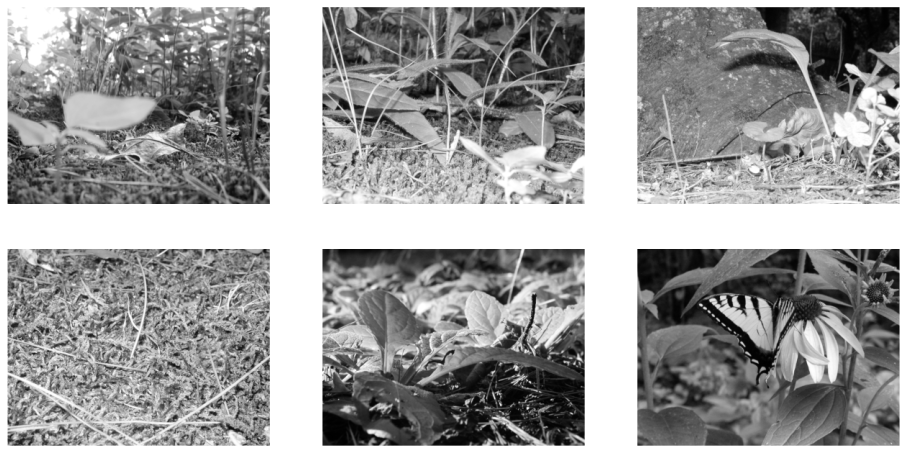
\includegraphics{/Users/bblais/Documents/Git/Amblyopia-Simulation/Manuscript/resources/fig-orig.svg}
\caption{Original natural images.}\label{fig:orig}
}
\end{figure}

\begin{figure}
\hypertarget{fig:logdog}{%
\centering
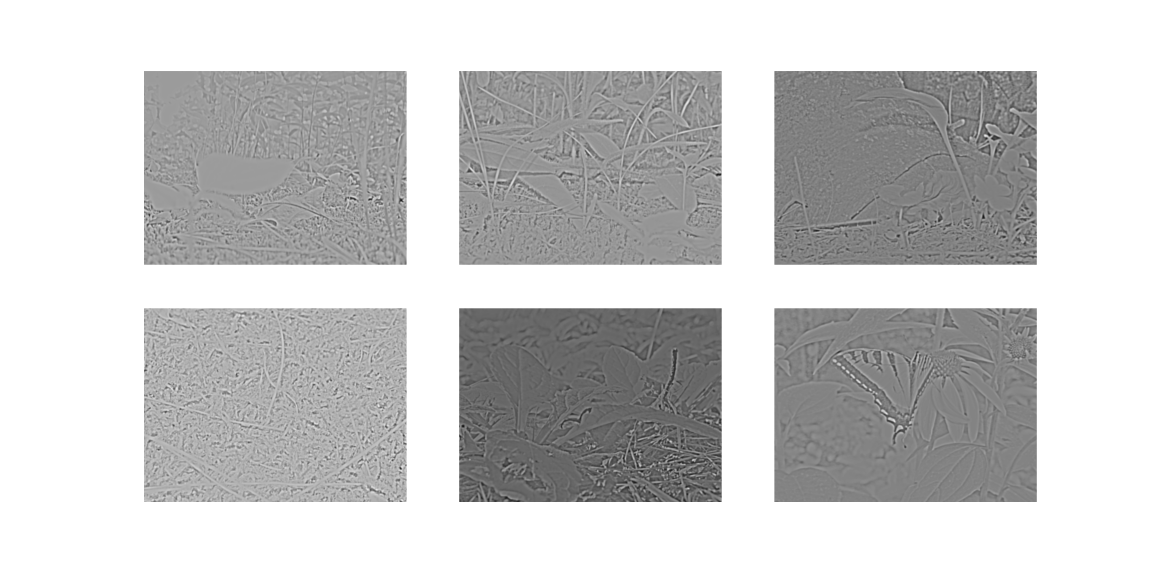
\includegraphics{/Users/bblais/Documents/Git/Amblyopia-Simulation/Manuscript/resources/fig-logdog.svg}
\caption{fig-logdog.svg}\label{fig:logdog}
}
\end{figure}

\hypertarget{references}{%
\section*{References}\label{references}}
\addcontentsline{toc}{section}{References}

\hypertarget{refs}{}
\begin{CSLReferences}{1}{0}
\leavevmode\vadjust pre{\hypertarget{ref-BCM82}{}}%
Bienenstock, E. L., Cooper, L. N., and Munro, P. W. (1982). Theory for
the development of neuron selectivity: Orientation specificity and
binocular interaction in visual cortex. \emph{Journal of Neuroscience},
\emph{2}, 32--48.

\leavevmode\vadjust pre{\hypertarget{ref-birch2013amblyopia}{}}%
Birch, E. E. (2013). Amblyopia and binocular vision. \emph{Progress in
Retinal and Eye Research}, \emph{33}, 67--84.

\leavevmode\vadjust pre{\hypertarget{ref-Gao_2018}{}}%
Gao, T. Y., Guo, C. X., Babu, R. J., Black, J. M., Bobier, W. R.,
Chakraborty, A., \ldots{} al., et. (2018).
\href{https://doi.org/10.1001/jamaophthalmol.2017.6090}{Effectiveness of
a binocular video game vs placebo video game for improving visual
functions in older children, teenagers, and adults with amblyopia}.
\emph{JAMA Ophthalmology}, \emph{136}(2), 172.

\leavevmode\vadjust pre{\hypertarget{ref-glaser2002randomized}{}}%
Glaser, S. R., Matazinski, A. M., Sclar, D. M., Sala, N. A., Vroman, C.
M., Tanner, C. E., et al.others. (2002). A randomized trial of atropine
vs patching for treatment of moderate amblyopia in children.
\emph{Archives of Ophthalmology}, \emph{120}(3), 268--278.

\leavevmode\vadjust pre{\hypertarget{ref-Holmes_2016}{}}%
Holmes, Jonathan M., Manh, V. M., Lazar, E. L., Beck, R. W., Birch, E.
E., Kraker, R. T., \ldots{} al., et. (2016a).
\href{https://doi.org/10.1001/jamaophthalmol.2016.4262}{Effect of a
binocular iPad game vs part-time patching in children aged 5 to 12 years
with amblyopia}. \emph{JAMA Ophthalmology}, \emph{134}(12), 1391.

\leavevmode\vadjust pre{\hypertarget{ref-holmes2016randomized}{}}%
Holmes, Jonathan M., Manh, V. M., Lazar, E. L., Beck, R. W., Birch, E.
E., Kraker, R. T., et al.others. (2016b). A randomized trial of a
binocular iPad game versus part-time patching in children 5 to 12 years
of age with amblyopia. \emph{JAMA Ophthalmology}, \emph{134}(12), 1391.

\leavevmode\vadjust pre{\hypertarget{ref-hubel1995eye}{}}%
Hubel, D. H. (1995). \emph{Eye, brain, and vision.} Scientific American
Library/Scientific American Books.

\leavevmode\vadjust pre{\hypertarget{ref-JeonEtAl1998}{}}%
Jeon, C. J., Strettoi, E., and Masland, R. H. (1998). {The major cell
populations of the mouse retina}. \emph{J Neurosci}, \emph{18}(21),
8936--8946.

\leavevmode\vadjust pre{\hypertarget{ref-Kelly_2016}{}}%
Kelly, K. R., Jost, R. M., Dao, L., Beauchamp, C. L., Leffler, J. N.,
and Birch, E. E. (2016).
\href{https://doi.org/10.1001/jamaophthalmol.2016.4224}{Binocular iPad
game vs patching for treatment of amblyopia in children}. \emph{JAMA
Ophthalmology}, \emph{134}(12), 1402.

\leavevmode\vadjust pre{\hypertarget{ref-Li:2015aa}{}}%
Li, S. L., Reynaud, A., Hess, R. F., Wang, Y.-Z., Jost, R. M., Morale,
S. E., \ldots{} Birch, E. E. (2015).
\href{https://doi.org/10.1016/j.jaapos.2015.08.003}{Dichoptic movie
viewing treats childhood amblyopia}. \emph{J AAPOS}, \emph{19}(5),
401--5.

\leavevmode\vadjust pre{\hypertarget{ref-SterlingEtAl1988}{}}%
Sterling, P., Freed, M. A., and Smith, R. G. (1988). {Architecture of
rod and cone circuits to the on-beta ganglion cell}. \emph{J Neurosci},
\emph{8}(2), 623--642.

\leavevmode\vadjust pre{\hypertarget{ref-wallace2018amblyopia}{}}%
Wallace, D. K., Repka, M. X., Lee, K. A., Melia, M., Christiansen, S.
P., Morse, C. L., and Sprunger, D. T. (2018). Amblyopia preferred
practice pattern{\textregistered}. \emph{Ophthalmology}, \emph{125}(1),
P105--P142.

\leavevmode\vadjust pre{\hypertarget{ref-xiao2022randomized}{}}%
Xiao, S., Angjeli, E., Wu, H. C., Gaier, E. D., Gomez, S., Travers, D.
A., et al.others. (2022). Randomized controlled trial of a dichoptic
digital therapeutic for amblyopia. \emph{Ophthalmology}, \emph{129}(1),
77--85.

\leavevmode\vadjust pre{\hypertarget{ref-xiao2020improved}{}}%
Xiao, S., Gaier, E. D., Mazow, M. L., Stout, A. U., Travers, D. A.,
Angjeli, E., \ldots{} Hunter, D. G. (2020). Improved adherence and
treatment outcomes with an engaging, personalized digital therapeutic in
amblyopia. \emph{Scientific Reports}, \emph{10}(1), 1--8.

\leavevmode\vadjust pre{\hypertarget{ref-de2007current}{}}%
Zárate, B. R. de, and Tejedor, J. (2007). Current concepts in the
management of amblyopia. \emph{Clinical Ophthalmology (Auckland, NZ)},
\emph{1}(4), 403.

\end{CSLReferences}

\end{document}
